\documentclass[12pt]{report}
\setlength{\parindent}{0pt}
\renewcommand{\baselinestretch}{1.3} 
\usepackage[a4paper, top=2cm, bottom=2cm]{geometry}
\usepackage[latin1]{inputenc}
\usepackage{setspace}
\usepackage{fancyhdr}
\usepackage{tocloft}
\usepackage{titlesec}
\usepackage{hyperref}
\usepackage{url}
\usepackage{indentfirst}
\usepackage{graphicx}
\usepackage{listings}
\usepackage{amsmath}
\usepackage[all]{xy}
\usepackage[font=footnotesize, labelfont={footnotesize,footnotesize}, margin=0cm]{caption}
\usepackage{algorithm} 
\usepackage{algpseudocode}
\usepackage[usenames,dvipsnames]{xcolor}
\usepackage{wrapfig}
\usepackage{graphicx}
\usepackage{booktabs}
\usepackage{siunitx}
\usepackage{amssymb}
\usepackage{tikz}
\usepackage{verbatim}
\usepackage{listings}
\usepackage{graphicx} 
\usepackage{subcaption}
\usepackage[algo2e]{algorithm2e}
\usepackage{booktabs}
\usepackage{paralist}
\usepackage{pbox} 





%\DeclareGraphicsExtensions{.png}

\fancypagestyle{plain} {
	\fancyhf{}
	\lhead[\rightmark]{\thepage}
	\rhead[\thepage]{\leftmark}
	\setlength{\parindent}{0pt} 
	\setlength{\parskip}{2ex}
}

\setlength{\parskip}{2ex}


\hypersetup{
    unicode=false,
    pdftoolbar=true,  
    pdfmenubar=true,     
    pdffitwindow=false,    
    pdfstartview={FitH},  
    pdftitle={TITLE GOES HERE},  
    pdfauthor={YOUR NAME GOES HERE},
    pdfsubject={SUBJECT GOES HERE},
    pdfnewwindow=true,  
    colorlinks=true,  
    linkcolor=black,  
    citecolor=black, 
    filecolor=black,  
    urlcolor=black  
}






\lstset{
	language=Haskell,
	basicstyle=\ttfamily, 
	identifierstyle=\ttfamily, 
	captionpos=b, 
	%frame=single, 
	numbers=left
}


\begin{document}

\pagestyle{empty}
\setcounter{page}{-100}

\date{} % the date has to be written onto the front page by hand
\title{\textbf{A fuzzy approach to Food Security through Microblogs }}
\author{\textbf{Alexander Buesser}\\
Computer Science\\
\'{E}cole Polytechnique F\'{e}d\'{e}rale de Lausanne\\
\\
I hereby declare that this paper is all my own work,\\
except as indicated in the text.\\
\\
Signature \line(1,0){200}\\
Date \line(1,0){40}/\line(1,0){40}/\line(1,0){40}\\
\\ 

\includegraphics[scale=0.2]{epfl_logo}}

\maketitle
%
% Dedication
%



\newpage

%
% Preface
%

\pagestyle{fancy}
\pagenumbering{roman}
\lhead[]{\thepage}
\rhead[\thepage]{}



\section*{Acknowledgements}


\newpage

%
% TOC
%

\tableofcontents

%
% Introduction
%

\setcounter{page}{1}
\chapter{Introduction}
\pagenumbering{arabic}







%\cleardoublepage
%\phantomsection
%\addcontentsline{toc}{chapter}{List of Tables}
%\listoftables

%\cleardoublepage
%\phantomsection
%\addcontentsline{toc}{chapter}{List of Figures}
%\listoffigures

%\cleardoublepage
%\phantomsection
%\addcontentsline{toc}{chapter}{Listings}
%\lstlistoflistings






\chapter{Data}
In this section we describe the filtering process of the tweets and the creation of three lexicons. The food lexicon contains tweets with food related terms (e.g. rice, wheat, milk) where the predictor lexicon contains tweets with factors influencing the price and supply of the goods (e.g. pricy, cheap, available) . The external factors lexicon similar to the second lexicon tries to capture the price and supply of different food commodities (e.g. oil, unemployment, flood). They differ that the former looks explicitly at keywords directly associated with food which give indication about the price fluctuation. The later is concerned with keywords describing external factors such as oil. We downloaded two TB of Tweets from the archive over a span of  October 2011 - September 2014.  The filtering process resulted with 1047698 food relevant tweets and 523549 tweets of influencing factors. 

Firstly, we detail an algorithm Hyperspace analogue to language (HAL)  \cite{lund96} which was used to find relevant keywords for our lexicon. We then describe our framework for retrieving food related keywords that build our food lexicon. The subsection Feature Definition describes how we define different predictor categories, followed by an illustration of the procedure we applied to retrieve predictor keywords. In Factors Keyword Selection we motivate the design of the external factors lexicon. Lastly we describe the filtering algorithm used to create our dataset. 


\section{Hyperspace analogue to language}

HAL creates a semantic space from word co-occurrences. For each word in some corpus HAL records the frequencies that other words in the corpus tend to occur before and after the word within a given window size. This is achieved  by storing a vector for each word with the number of co-occurences of every other word in the corpus. Hence if our corpus contains N different words the resulting HAL space would be an N x N square matrix of co-occurences. For each appearance of a word in the corpus, these co-occurnence vectors are updated. It is important to note that only the context before the word is recorded because the context after the word will appear in the column in the matrix that corresponds to that word. For each co-occurence HAL applies a scoring function. Words that appear closer receive an inversely proportionated score to its distance. To illustrate the idea Table \ref{tab:halex} gives an example of a simple sentence \emph {"The horse raced past the barn fell."} with a sliding window of five. 

Following the creation of the matrix we take both the column and row vector of a word, thus including both the preceding and following contexts of the words, and concatenate them. The result is a meaning vector that now can be compared. This can be simply done by using some distance measure. In this paper we use the cosine similarity. 

\begin{table}[h]
\centering
\begin{tabular}{ c c c c c c} \toprule
  & Barn & Horse &  Past & Raced & The \\ 
  \hline
 Barn &  & 2 &  4 & 3 & 6 \\ 
 Fell & 5 & 1 &  3 & 2 & 4 \\ 
 Horse &  &  &   &  & 5 \\ 
 Past &  & 4 &   & 5 & 3 \\ 
 Raced &  & 5 &   &  & 4 \\ 
 The &  & 3 &  5 & 4 & 2 \\ 
   \bottomrule
\end{tabular}
\caption{Toy example of HAL}
\label{tab:halex}
\end{table}

Let's consider the first row.  \emph{"The"} precedes \emph{"Barn"} twice. Once within a distance of five and the other time it directly precedes the word  \emph{"Barn"}. Hence that cell receives a score of five for the proximate one and a score of one for the word further away resulting in a final score of six. 




\section{Food Keyword Selection}

The filtering of the dataset was initially performed with a simple list of food related keywords. To avoid ambiguities we will refer to the initial keyword list as $K_i$. As a first source for our set $K_i$ we used the most common traded food commodities as it would easily allow us to verify our results using the price dataset made available by IMF \footnote{http://www.imf.org/external/np/res/commod/index.aspx}. We further decided to include the ten most important staple foods that feed the world as defined by Allianz\footnote{http://knowledge.allianz.com/demography/health/?767/the-worlds-staple-foods}. Tweets were retrieved through exact term matching i.e. a tweet containing foods would not match on the keyword food where the reverse is also true. We mimic the term matching twitter performs. In the initial round we aimed for maximum coverage and hence avoided further filtering steps. The result was a collection of 1047698 tweets posted by 949085 user. 


Looking at the distribution of the food related tweets we realised that we would have to categorise our lexicon in order to have sufficient data for further analysis. Where global keywords such as food are highly represented, more specific keywords such as beef only occur very infrequently. Other then the sparsity of the data we also have the problem of ambiguous keywords. Soy is such a keyword that refers in english to the "bean" and in spanish to the verb "to be". To create categories we chose to mimic the categorisation of the FAO  \footnote{http://www.fao.org/worldfoodsituation/foodpricesindex/en/}. The FAO tries to measure the overall food fluctuation by five different food categories namely \emph{meat, dairy products, cereals, vegetable oil} and \emph {sugar}. The weighted average of those five categories defines the international food price index. We additionally created a further category named \emph{Other Food of Interest}. This category contains general keywords (e.g. food, dinner or lunch) and food keywords that can not be assigned to one of the five categories but frequently occur (e.g. coffee, tea). To be considered frequently the set of tweets containing the keyword needs to be $> 1\%$ of the total sample. Those six subsets  $s$ are $\in K_e$. C is a fictional set that contains the five categories \emph{meat, dairy products, cereals, vegetable oil, sugar}  each building a subset containing all possible food items belonging to a specific category (e.g. the subset dairy would contain all possible dairy products). If the following relationship holds  $k \in C$ for any  keyword $k \in K_i$, we consdier $k \in K_e$. For all keyword $k \notin C$ the condition of it being frequent is evaluated and if true added to $K_e$.  Food commodities that could not be assigned to one of the six categories were discarded. Upon manual examination of the dataset we realised that people are much more likely to talk about a specific food product rather then the raw material. Cereals are not a public interest, however products such as bread or flower occur much more frequently. The set $K_e$  was further enriched by using food products that have been identified by \cite{AbbarMW14} in set $K_f$ only $\forall$ $k   \in K_f$ that are also $\in C$ . To further improve our coverage of the six food categories we filtered for synonyms and contextual similar words using HAL. What we mean by contextual similar and how HAL retrieves those keywords is further described in Section 3.3.1.

\subsection{Our approach}

We took several  steps in order to improve our detection of the desired food commodities. $K_e$ was created as follows: 
\begin{description}
  \item[1.)] We add all keywords $k \in K_i$ to  $K_e$ only if $k \in C $ or $k$ is frequent 
  \item[2.)] Further add all keywords $ k \in K_f$ to $K_e$ only if $k \in C$
  \item[3.)] From a subsample of 10\% we create a HAL space with all keywords that occur $> 100$. $\forall c \in C $ we pick the keyword $k\in K_e$ that most frequently occurs and retrieve the top 500 similar terms. We hand select those that are $\in C$.
\end{description}

% We took several  steps in order to improve our detection of the desired food commodities. The first step we took was a simple context analysis. The basic premise our approach relies on is that words with similar meaning repeatedly occur with similar words preceding and following it. We took a sample of 10 \% and counted the frequency of the 500 most occurring nouns and hand selected those unambiguously related to food. Looking at the distribution of the food related tweets \textbf{ \ref{fig:keywordDistribution}} we realised that we would have to categorise our lexicon in order to have sufficient data for further analysis.
 
The keyword set $K_e$ was used to perform exact term matching on the tweets collected from the archive. The resulting set of keywords in $K_e$ forms our Food Lexicon.  



 
\begin{table}[h]   
\centering
\scriptsize 
\begin{tabular}{p{1.3cm}|p{10.7cm} rlr}\toprule
\pbox{1.3cm}{Lexicon / \\ Subset $s$\\} & Keywords (i: from initial set, e: from $K_f$ , h: from HAL space )  \\
\hline
& & \\
\pbox{1.3cm}{$K_i$ \\Food } & \pbox{10.7cm}{  meal (i), meals (i) ,food (i), foods (i), wheat (i), rice v, maize (i), carley (i), soybean (i), soy (i), meat (i) , beef (i), cattle (i), chicken (i), poultry (i), lamb (i), swine (i), pork (i), fish (i), seafood (i), shrimp (i), salmon (i), sugar (i), bananas (i), oranges (i), coffee (i), cocoa (i), tea (i), milk (i), yams (i), cassava (i), potatoes (i), sorghum (i), plantain (i), nuts (i), onion (i), salt (i), egg (i), dairy (i), cereals (i)  }    \\
& & \\
 

\hline
\hline

& & \\
\pbox{1.3cm}{$K_e$ \\ Meat }  & \pbox{10.7cm}{ meat (i), lamb (i), pork (i), swine (i), chicken (i), poultry (i), beef (i),  sausage (e), rib (e), pastrami (e), kidney (e), liver (e), ham (e), bacon (e), chorizo (e), salami (e), sheep (e), boeuf (e), oxen (e), kine (e), steak (e), cow (e), brisket (e), veal (e), tenderloin (e), sirloin (e), poulet (e), volaille (e), hot dog (h), hamburgers (h),  meatballs (h), burgers (h), goat (h), cattle v, turkey (h), pig (h)}  \\
 & & \\
\hline

& & \\
\pbox{1.3cm}{$K_e$ \\Cereals }  & \pbox{10.7cm}{ wheat (i), atta (i), starch (i), farina (i), bran (i), ethanol (i), biofuel (i), rice (i), corn (i), maize (i), ravioli (e),  barley (e), scotch (e), whisky (h), oat (h), bread (h), flour (h), gluten (h), pasta (h), noodles (h), beer (h)  }  \\
& & \\

\hline

& & \\
\pbox{1.3cm}{$K_e$  \\Oil }  & \pbox{10.7cm}{ coconut oil (i), corn oil (i), olive oil (i), palm oil (i),peanut oil (i), sunflower oil (i), rapeseed oil (i), 
                                                              safflower oil (i),soybean oi (i), sunflower oil (i), soybeans (i), soya (i), soy sauce (i), soja (i)  }  \\
& & \\

\hline

& & \\
\pbox{1.3cm}{$K_e$ \\ Sugar }  & \pbox{10.7cm}{ sugar (i),  sugarcane (i), syrup (e), energy drink (e), cola (e), chocolate (e), nestle (e), cookies (h), cupcakes (h) }  \\
& & \\
 \hline                                                      

& & \\
\pbox{1.3cm}{$K_e$  \\ Dairy }  & \pbox{10.7cm}{ dairy (i), egg (i), milk (i), kefir (e) , butter (e), yogurt (e), quark (e), mozzarella (e), cheddar (e), parmesan (e),  
 		             buttermilk (e), ricotta (e), feta (e), romano (e), provolone (e), colby (e), edam (e), eggnog (e), pimento (e), 
		             cheshire (e), roquefort (e), icecream (h), milkshake (h), cheese (h), cream (h)} \\
& & \\
           
\hline

& & \\
\pbox{1.3cm}{$K_e$ \\ Other}  & \pbox{10.7cm}{ meal (i), meals (i), food (i), foods (i), fish (i) , prawn (i), seafood (i), salmon (i), tea (i), coffee (i),  dinner (h), lunch (h), breakfast (h), dish (h), cuisine (h)}  \\
& & \\

 \bottomrule

\end{tabular}
\caption{ A summary of the evolution of our Food Lexicon}
\label{tab:abc}
\end{table}
 



\section{Predictor Keyword Selection}

From our basic food lexicon we proceeded to extract features that we could use to predict the price and the global food security index. The FAO measures food security based on four dimensions namely \emph{Access, Availability, Stability} and \emph{Utilisation}. Where \emph{Access} mostly captures the supply of food, \emph{Availability} is concerned with the affordability of the basic goods. \emph{Utilisation} captures the nutritional value of the food and lastly \emph{Stability} is a measure of the other three dimensions over time. For food security objectives to be realised, all four dimensions must be fulfilled simultaneously \cite{fao2008}. 


To model food security we focus our work on those four dimension namely \emph{Access, Availability, Utilisation} and \emph{Stability}. Together those predictor categories build the set $C_p$. Attempts have been made to capture Availability by the UN \cite{ungp2013}. Bellow we will describe an algorithm that builds on the UN's idea namely selecting tweets that match a certain pattern of keyword categories. 


We define the predictor category \emph{Access} by looking for tweets containing price as a keyword as in \cite{ungp2013} but improve the recall by including synonyms of price that appear in the same context. \emph{Availability} was defined in similar fashion by matching keywords that appear in the context of food availability. Unlike \cite{AbbarMW14} we don't measure food Utilisation by observing the exact diet but capture the people's food needs. Lastly as a measure of \emph{Stability} we focused our attention on economic stability. Keywords in the context of  poverty were selected to match this predictor category. 

\subsection{Motivating a semantic approach}
\label{subsec:hal}

In this section we try to comprehend which words are associated with the above mentioned categories in $C_p$. More specifically what words are represented in the context of food supply, food price, food needs and food poverty. To achieve this we need a plausible methodology for representing the meaning of a word. The reason why we analyse the context of a word is to identify new words that have a similar meaning or given the same context express the same thing. The later is concerned with identifying synonyms where as the former looks at contextual similarity. For example let's look at the word \emph {"mold"} and  \emph {"available"}. Those two words seem unrelate but given the context of food the express the same thing.  Namely an abundance of food. Through the role  of the context they posses elements of items similarity but by themselves they would never be considered words with similar meaning. It's important to stress that they are not similar because they occur frequently locally but because the occur frequently in similar sentential context. Burgess et al. \cite{burgess98} argues that a simple local co-occurence analysis misses to capture a lot of relationships. For example the word street and road are basically synonyms however the seldomly locally co-occur. They do, however occur in the same contexts. This observation motivated us to deviate from the commonly used co-occurence analysis an take a step further to improve the precision of our filtering framework. 



\subsection{Our approach}

We use a large text corpus of around 23860931 words. As a source we used a random sample of 10 \% from our food related tweets. Our corpus of food related tweets has a number of appealing properties as it covers a large vocabulary centered around food. Unlike most corpras that represent formal business reports or specialised dictionaries our food corpus represents everyday speech. This gives us a closer proximation on how people would talk in the context of our predictor categories. 

The vocabulary of the HAL model contains 14084 words. The initial set of words in our corpus was filtered only to contain those words that appear at leat 100 times. Words occurring infrequent were discarded as well as stop words and punctuations. We shall refer to this set of words as $F_c$. Using the words $w \in F_c$ we produced a 14084 by 14084 matrix wit the co-occurences within a window size of five. Since vector similarity measures are sensitive to the magnitude of the vectors we normalized all the vectors to a constant length. Once the HAL space was created we performed the following steps to retrieve the desired keywords for our four categories. 


\begin{description}
  \item[1.)] $\forall k \in K_e$ choose the keyword k with the highest occurrence. Let's call it $k_{max}$  
  \item[2.)] $\forall w \in F_c $ perfomre a similarity meassure with $k_{max}$
  \item[3.)] Retrieve the 500 most similar words and handselect one word for each element of $C_p$ (e.g. since we have four categories the result should be four words)
  \item[4.)] For each of those handselected words  apply HAL and compare it $\forall$ $w \in F_c $
  \item[5.)] For each predictor category retrieve the 500 most similar words and manually select relevant keywords. 
  \end{description}

The high-level intuition of this procedure is as follows. The first step will give us the most prominent food term. This is most likely going to be something general such as the keyword \emph{"Food"}. Step 2 and 3 will allow us the identify the most contextual similar keywords for each category. So the keyword is retrieved that is most likely used to describe supply in the context of food. In step 4 and 5 we aim to retrieve similar words that could describe supply but maybe appear more frequently in different contexts. In other words we aim to find synonyms here.   

\subsection{Results}


Other then the words for our categories of interest HAL highlights some clear topics associated around food. As expected other contextual similar words were other food items building the clear majority of the retrieved words. Interestingly there was also a high percentage of country names in the retrieved results. Looking more closely at the retrieved countries we could see that most of them have a clear association to food. Where the majority of the retrieved countries such as Thailand, Bali or the cities Sinagpore and Paris are considered to be famous holiday destinations for food lovers other retrieved countries such as Pakistan, Syria, Jakarta India or the Philippines are cities with a clear history of food insecurity and political unrest. 

Words that fell into our categories of interests were words such as available, profit, price, sustainability, progress, sales,  war, easy. The four words we used to model the predictor categories were \emph{available} for supply, \emph{price} for price, \emph{children} for poverty and \emph{help} for needs. In table 


 
\begin{table}[h]   
\centering
\scriptsize 
\begin{tabular}{p{1.3cm}|p{10.7cm} rlr}\toprule
\pbox{1.3cm}{Lexicon / \\ Subset $s$\\} & Keywords (i: from initial set, e: from $K_f$ , h: from HAL space )  \\
\hline

& & \\
\pbox{1.3cm}{$Food$ \\ Supply }  & \pbox{10.7cm}{  \emph{available}, giveaway, coupons, , growth, sustainability, nomnom, receive, indonessia, berlin, program, institute, survey, news, farming, journal, strategy, price, india, check, canada, production, campaign, protection, imports, launched, rating, storage, nutrition, restaurant, resources, trends, container, stall, government, distribution, processing, impact, policy, consumption, stores, exports, opportunities, harvest,price,savings,discount, budget, profits, increase, rise,relief
}  \\
 & & \\
\hline
& & \\
\pbox{1.3cm}{$Food $ \\Price }  & \pbox{10.7cm}{
\emph{price}, issue, india, coupon, health, children, news, malaysia, discount, benefit, syria, asia, indonessia, philippines, grothw, dubai, consumer, campaign, sold, agriculture, available
, sustainability, thailand, farming, markets, harvest, program, success, foundation, crops, politics, demand, purchase disaster, rates, safe, cost, association, nutrition, nation, sponsored, fundraiser, protest, deal, giveaway, growing, dangerous, threat future, programs, fighting, farms, consumers, support, jakarta, pakistan, africa, curtesy, poverty, exports drought,  funding, bill, summit, delhi, rating, priced, justice, avoid }  \\
& & \\
\hline
& & \\
\pbox{1.3cm}{$Food $ \\Poverty }  & \pbox{10.7cm}{\emph{children},  community, source, future, issue, safe, project, growing, support, benefit, india, health, asia, baby, government, dangerous, area, agriculture, politics, poverty, cultures, obesity, tax, changes, program, freedom, price, impact, news, report, nutrition, help, country, syria, sustainability, philippines, success, awesome, farm, donate, diet, foundation, indonesia, summit, supplies, israel, farms, farming, kills, cash, crops, confernece, projects, seeking, nation, fight, protection, courtesy  }  \\
& & \\
\hline
& & \\
\pbox{1.3cm}{$Food $ \\Needs }  & \pbox{10.7cm}{ 
\emph{help},power, amazing, thanks, future, children, beyond, yummy, issue, death, killing, helping, brilliant, delicious, awesome, tasty, freedom, kill, needed, nice, healthier, benefits helps, feeding, love, tax often, health, incredible, politics, destroy, expensive, increase, yum, heavenly, trash, necessary, cheap, enjoy, smiling, struggle, disaster, stress   }  \\
& & \\





\bottomrule

\end{tabular}
\caption{ Keywords of Predictor Categories}
\label{tab:abc}
\end{table}
 
 \newpage

\section{Factor Keyword Selection}






\section{Filtering}

Following the creation of the four categories we used polarities to model the price variation. For example, the category \emph{"price"} has two polarities: \emph{"high"} and \emph{"low"}. In \cite{hum14} we worked on a filtering mechanism to extract relevant tweets and to assign them to the relevant polarities.  In order to achieve this goal, a prediction lexicon with a total of four categories was built (\emph{ "price", "poverty", "needs", "supply"}), let's call it $D$.

Then, for each tweet a feature vector is built, representing the amount of words from each category and polarity. Several cases have to be taken into account. First of all, a word may be not in its base form ("price" $\to$ "prices", "increase" $\to$ "increasing"), which will prevent an incoming word from matching one from $D$. Therefore, we use stemming technique to reduce each word to its stem (or root) form. Another problem is misspelled words ("increase" $\to$ "incrase", "incraese"), and for tweets it happens more than usual due to widespread use of mobile devices with tiny keyboards. To allow for an efficient execution of the filtering  we decided to use a simple approach which involved computing edit distances between a given word and words from predictor categories dictionary ($D$).
For each given word $w$ we compute its stem $s$ and then edit distance (also known as Levenshtein distance) to each word (stem) from $D$.
After that, we choose the stem with minimal edit distance, and check if the resulting number of "errors" (which is equal to distance) is excusable for the length of word $w$. For example, we don't allow errors for words of length 5 or less, only one error is allowed for lengths from 6 to 8, etc. If everything is alright, then the suggestion is returned, otherwise the word is discarded. 

Furthermore we had to account for negation words, which subverts the meaning: "increases" $\to$ "doesn't increase", "have food" $\to$ "have no food".  To deal with this problem, we employed the following method: we added a special 'negation' category with a list of negation words ("not", "haven't", "won't", etc.), and if there is a word with "negative" category before some relative word (to be more precise, within some constant distance from it, say 2), then we change the polarity of relative word's category. For example, if a word is from category "poverty" and has a "high" polarity (e.g. "starving"), then a negative category word right before it (such as "aren't") will turn the polarity to "low".


\section {Discussion}




\chapter{Analysis}

\section{General Stats}

We see in the bellow Figure \textbf{\ref{fig:tpu}} that the distribution of the number of tweets per user follows a power law where a lot of individuals have sent only a few tweets about the subject and only a small number of users have sent a large amount of tweets. 


 
 \begin{figure}[H]
\centerline{ \noindent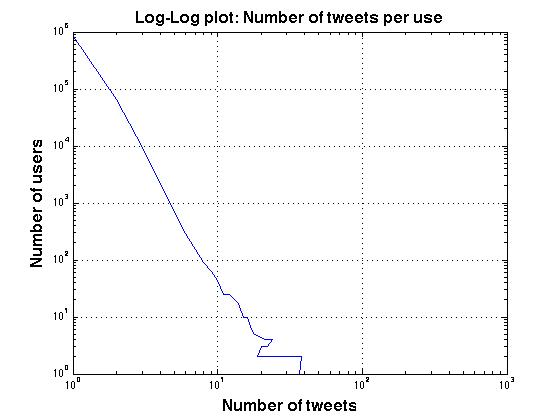
\includegraphics[width=1\textwidth]{img/anal/loglog_users_tweets}}
 \caption{Distribution of Tweets per User}
 \label{fig:tpu}
\end{figure}

  \begin{figure}[H]
\centerline{ \noindent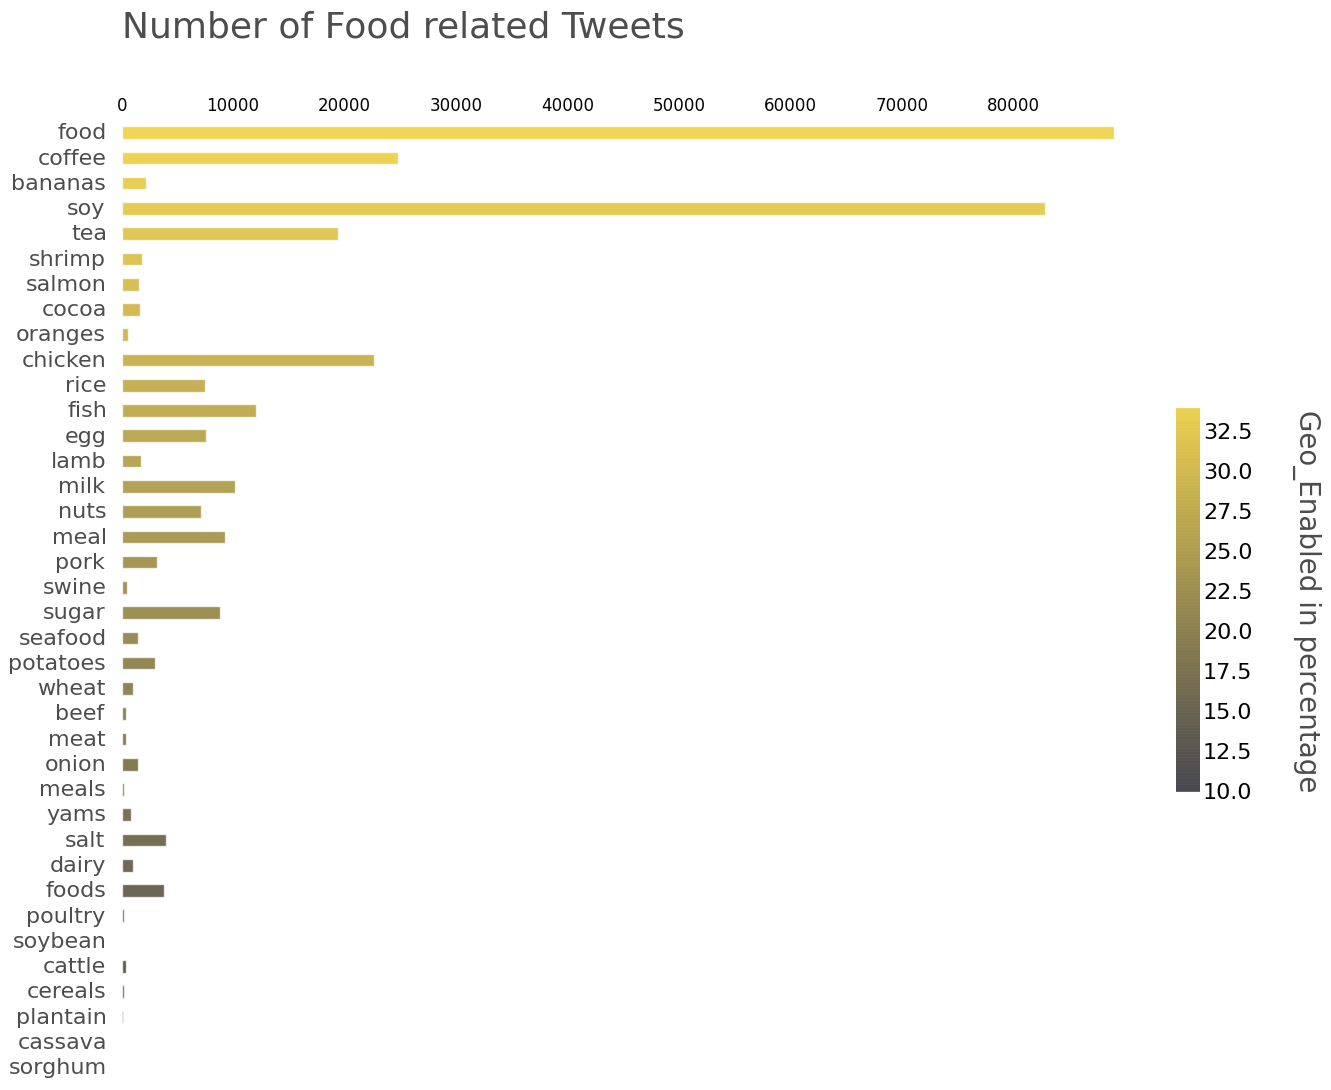
\includegraphics[width=1\textwidth]{img/anal/n_food_tweets}}
 \caption{Keyword Distribution}
 \label{fig:keywordDistribution}
\end{figure}
 


%
% liography
%

\cleardoublepage
\phantomsection
\addcontentsline{toc}{chapter}{Bibliography}

\bibliographystyle{plain}
\bibliography{bibDatabase}



\cleardoublepage
\phantomsection
\chapter*{Appendix}

\section{Processing and Storage}

 To facilitate the storage and processing of this large amount of data we used an AMD supercomputer with 64 cores. Inspired by the  map reduce paradigm we split the dataset into 64 parts and assigned each to a single core. To efficiently use the hardware resources we manually controlled for the memory assignment using numactl. As illustrated in\textbf{ \ref{fig:dataProcessing}} eight cores directly access one out of eight memory blocks. Each dataset was filtered in parallel reducing the 64 dataset to two lexicons. 

 \begin{figure}[H]
\centerline{ \noindent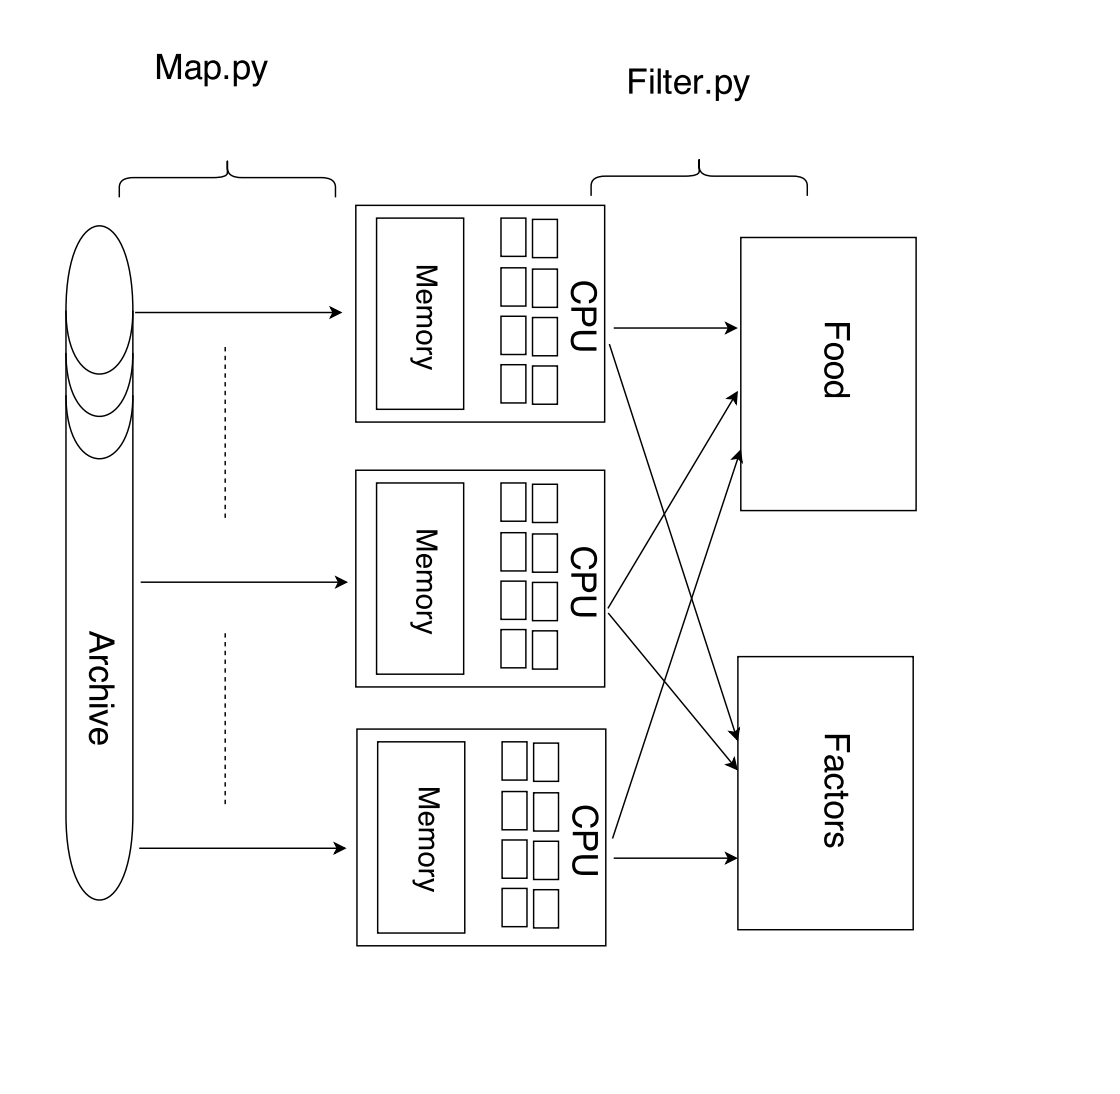
\includegraphics[width=1\textwidth]{img/abs/hw_model}}
 \caption{Dada Processing}
 \label{fig:dataProcessing}
\end{figure}



\textbf{function get\_category(w):}

\indent
\begin{algorithm}[H]
Compute a stem $s$ from $w$ \par
Check if $s$ is present in $RI$.

  \eIf{yes}{\textbf{return} the corresponding tuple.
   }{
		ask spell checker for a suggestion \par
		is suggestion stem returned? \par
		\eIf{yes}{
			\textbf{return} the corresponding tuple from $RI$
		}{
			\textbf{return} None;
		}
  	}
% \caption{Algo}
\end{algorithm}
\noindent \\





 \begin{figure}[H]
\centerline{ \noindent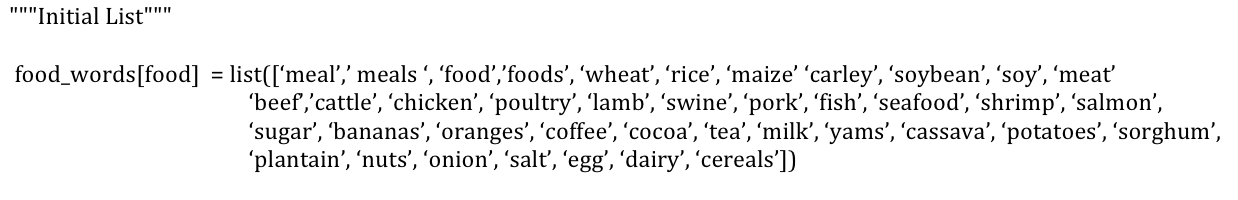
\includegraphics[width=1\textwidth]{img/abs/ini_lex}}
 \caption{Keywords: Food Lexicion}
 \label{fig:flex}
\end{figure}

 \color{red} Initial Keywords: \\
 \color{blue}Extended Keywords:  \\
\color{green}Hal Keywords:  \\


 \begin{figure}[H]
\centerline{ \noindent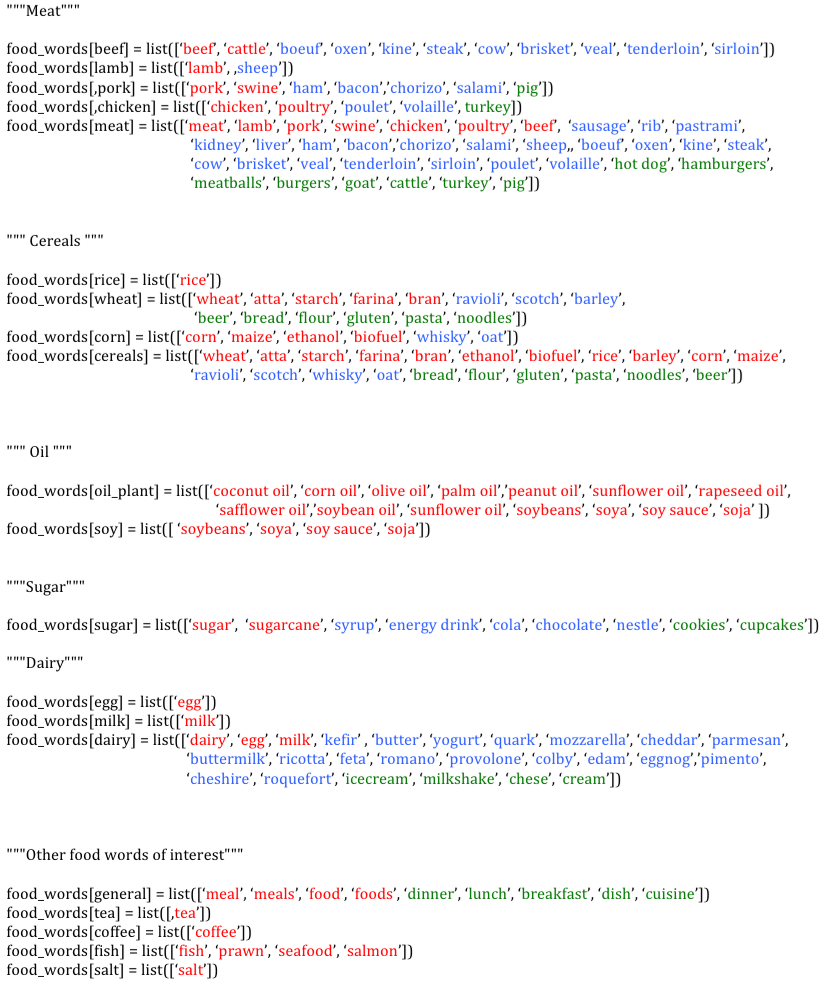
\includegraphics[width=1\textwidth]{img/abs/hyrach_lex}}
 \caption{Keywords: Food Lexicion}
 \label{fig:flex}
\end{figure}




\end{document}